\section{Capítulo 6 -- Funções e procedimentos}

Os programas dos capítulos anteriores cabiam inteiros no \texttt{main}. Programas reais têm milhares ou milhões de linhas, e ninguém consegue entender, testar ou corrigir um bloco desse tamanho de uma vez. A saída é a mesma que usamos para qualquer problema grande: dividir em partes menores, cada uma com uma tarefa clara. Em programação, essas partes são os \textbf{subprogramas}: as \textbf{funções}, que calculam e devolvem um valor, e os \textbf{procedimentos}, que executam uma tarefa sem devolver nada. Neste capítulo você vai aprender a criar os seus, a passar dados para eles e a entender o que acontece na memória a cada chamada.

\subsection{6.1 Dividir para conquistar}

Você já usa funções desde o Capítulo 3, mesmo sem ter escrito nenhuma. A \texttt{sqrt}, que calcula a raiz quadrada, e a \texttt{pow}, que calcula potências, são funções prontas da biblioteca \texttt{<cmath>}:

\begin{codigo}
\begin{Verbatim}[breaklines=true, breaksymbolleft={}, fontsize=\footnotesize]
#include <iostream>
#include <cmath>       // sqrt, pow
using namespace std;

int main() {
    double r = sqrt(49.0);       // 7
    double p = pow(2.0, 10);     // 1024
    cout << r << " " << p << endl;
    return 0;
}
\end{Verbatim}
\end{codigo}

Para usar a \texttt{sqrt}, você não precisa saber como ela calcula a raiz: basta saber o que ela recebe (um número) e o que devolve (a raiz). Essa ideia, usar algo pelo que ele faz sem se preocupar com como faz, chama-se \textbf{abstração}, e é o principal ganho de dividir um programa em subprogramas. Há outros:

\begin{itemize}
  \item \textbf{Reaproveitamento}: o código escrito uma vez é chamado quantas vezes for preciso, em vez de ser copiado e colado.
  \item \textbf{Manutenção}: um erro corrigido na função fica corrigido em todos os lugares que a usam.
  \item \textbf{Teste}: cada função pode ser testada sozinha, com poucos casos, antes de ser combinada com as outras.
  \item \textbf{Legibilidade}: um \texttt{main} que só chama \texttt{lerNotas}, depois \texttt{calcularMedia} e por fim \texttt{mostrarResultado} se lê quase como um texto.
\end{itemize}

Dividir um programa em partes independentes chama-se \textbf{modularização}. A regra prática é simples: cada subprograma deve fazer \textbf{uma única tarefa}, e seu nome deve dizer qual é.

\subsection{6.2 Funções: recebem dados e devolvem um resultado}

Uma função tem um \textbf{cabeçalho}, que diz o tipo do resultado, o nome e os dados que ela recebe, e um \textbf{corpo}, entre chaves, com os comandos que calculam o resultado.

\begin{center}
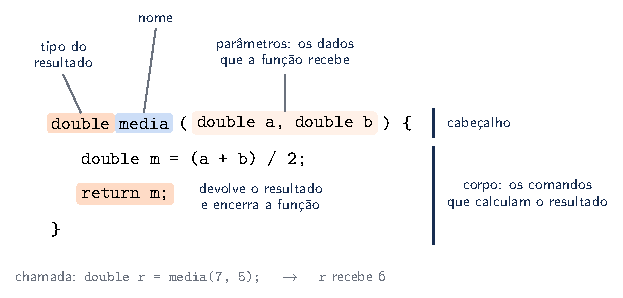
\includegraphics[width=0.85\linewidth,keepaspectratio]{imagens/capitulo-06_anatomia.pdf}
\end{center}

Os \textbf{parâmetros} são variáveis declaradas no cabeçalho, que recebem os valores passados na chamada. Esses valores são os \textbf{argumentos}. Na chamada \texttt{media(n1, n2)}, o parâmetro \texttt{a} recebe o valor de \texttt{n1} e o \texttt{b}, o de \texttt{n2}: a correspondência é pela \textbf{posição}, não pelo nome. O comando \texttt{return} encerra a função e entrega o resultado a quem a chamou.

\begin{codigo}
\begin{Verbatim}[breaklines=true, breaksymbolleft={}, fontsize=\footnotesize]
#include <iostream>
using namespace std;

double media(double a, double b) {
    double m = (a + b) / 2;
    return m;
}

int main() {
    double n1, n2;
    cout << "Duas notas: ";
    cin >> n1 >> n2;
    double resultado = media(n1, n2);
    cout << "Média: " << resultado << endl;
    cout << "Média de 8 e 5: " << media(8, 5) << endl;   // 6.5
    return 0;
}
\end{Verbatim}
\end{codigo}

A chamada \texttt{media(n1, n2)} é uma expressão, como \texttt{n1 + n2}: o resultado pode ser guardado em uma variável, mostrado direto no \texttt{cout} ou usado dentro de outra conta, como em \texttt{media(n1, n2) >= 6}. Os argumentos também podem ser expressões ou valores literais, como em \texttt{media(8, 5)}.

Em Portugol, a função é declarada entre a seção \texttt{var} do algoritmo e o \texttt{inicio}, com \texttt{funcao ... fimfuncao}. O tipo do resultado vem depois dos parâmetros, e o resultado é devolvido com \texttt{retorne}:

\begin{codigo}
\begin{Verbatim}[breaklines=true, breaksymbolleft={}, fontsize=\footnotesize]
algoritmo "MediaComFuncao"
var
   n1, n2, resultado: real

funcao media(a, b: real): real
var
   m: real
inicio
   m <- (a + b) / 2
   retorne m
fimfuncao

inicio
   escreva("Duas notas: ")
   leia(n1, n2)
   resultado <- media(n1, n2)
   escreval("Média: ", resultado)
fimalgoritmo
\end{Verbatim}
\end{codigo}

\subsubsection{Mais de um return}

O \texttt{return} encerra a função \textbf{imediatamente}, mesmo no meio de um laço. Por isso, uma função pode ter vários, um para cada caso. O teste de número primo do Capítulo 5 fica mais curto como função: assim que um divisor aparece, a resposta já é conhecida.

\begin{codigo}
\begin{Verbatim}[breaklines=true, breaksymbolleft={}, fontsize=\footnotesize]
#include <iostream>
using namespace std;

bool ehPrimo(int n) {
    if (n < 2) return false;           // 0 e 1 não são primos
    for (int d = 2; d * d <= n; d++) {
        if (n % d == 0) return false;  // achou divisor: sai já
    }
    return true;                       // nenhum divisor
}

int main() {
    cout << "Primos até 50:";
    for (int n = 1; n <= 50; n++) {
        if (ehPrimo(n)) cout << " " << n;
    }
    cout << endl;   // 2 3 5 7 11 13 17 19 23 29 31 37 41 43 47
    return 0;
}
\end{Verbatim}
\end{codigo}

Compare com o Capítulo 5: lá, o teste usava uma variável \texttt{primo} e um \texttt{break}. Aqui, o \texttt{main} só pergunta ``\texttt{n} é primo?'' e não precisa saber como a resposta é obtida. Funções que respondem sim ou não costumam ter nomes como \texttt{ehPrimo}, \texttt{ehPar} ou \texttt{estaAprovado}, e devolvem \texttt{bool}.

Toda função que não é \texttt{void} precisa devolver um valor em \textbf{todos} os caminhos. Se algum caminho chegar ao fim do corpo sem um \texttt{return}, o resultado é indefinido, e o g++ avisa com \texttt{-Wall}.

\subsection{6.3 Procedimentos: executam uma tarefa}

Nem todo subprograma calcula um valor. Mostrar um cabeçalho, desenhar uma linha ou imprimir um relatório são tarefas que não têm resultado a devolver. Esses subprogramas são os \textbf{procedimentos}. Em C++, um procedimento é uma função com tipo de retorno \texttt{void} (``vazio''):

\begin{codigo}
\begin{Verbatim}[breaklines=true, breaksymbolleft={}, fontsize=\footnotesize]
#include <iostream>
#include <string>
using namespace std;

void linha(int tamanho, char simbolo) {
    for (int i = 0; i < tamanho; i++) {
        cout << simbolo;
    }
    cout << endl;
}

void cabecalho(string titulo) {
    linha(30, '=');
    cout << titulo << endl;
    linha(30, '=');
}

int main() {
    cabecalho("Relatório de notas");
    cout << "Ana     8.5" << endl;
    cout << "Bruno   6.0" << endl;
    linha(30, '-');
    return 0;
}
\end{Verbatim}
\end{codigo}

Repare que \texttt{cabecalho} chama \texttt{linha}: subprogramas podem (e devem) usar outros subprogramas. Um procedimento não tem \texttt{return} com valor, mas pode usar \texttt{return;} sozinho para terminar mais cedo, por exemplo quando recebe um dado inválido.

Em Portugol, o procedimento é escrito com \texttt{procedimento ... fimprocedimento}, sem tipo de retorno:

\begin{codigo}
\begin{Verbatim}[breaklines=true, breaksymbolleft={}, fontsize=\footnotesize]
algoritmo "Relatorio"

procedimento linha(tamanho: inteiro)
var
   i: inteiro
inicio
   para i de 1 ate tamanho faca
      escreva("-")
   fimpara
   escreval("")
fimprocedimento

inicio
   linha(30)
   escreval("Relatório de notas")
   linha(30)
fimalgoritmo
\end{Verbatim}
\end{codigo}

A diferença entre os dois tipos de subprograma aparece também na chamada. Uma função é usada \textbf{como um valor}, dentro de uma expressão: \texttt{x <- media(a, b)}. Um procedimento é usado \textbf{como um comando}, sozinho na linha: \texttt{linha(30)}.

\subsection{6.4 O que acontece em uma chamada}

Quando o programa chama uma função, quatro coisas acontecem, nesta ordem:

\begin{enumerate}
  \item os argumentos são avaliados e seus valores são \textbf{copiados} para os parâmetros;
  \item o programa salta para o início do corpo da função, e anota para onde deve voltar;
  \item o corpo é executado, com seus próprios parâmetros e variáveis;
  \item no \texttt{return} (ou no fim do corpo), o resultado é entregue, as variáveis da função deixam de existir e o programa continua do ponto onde parou.
\end{enumerate}

Para organizar isso, o computador usa uma região da memória chamada \textbf{pilha de chamadas}. Cada chamada ganha um \textbf{registro de ativação}, um espaço com seus parâmetros e variáveis locais, empilhado sobre o de quem a chamou. Quando a função termina, seu registro é desempilhado. A figura mostra a pilha durante a chamada \texttt{media(n1, n2)}, com as notas 7 e 5:

\begin{center}
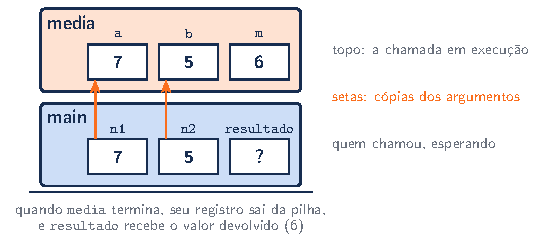
\includegraphics[width=0.85\linewidth,keepaspectratio]{imagens/capitulo-06_pilha.pdf}
\end{center}

Duas consequências importantes vêm daí. Primeiro, \texttt{a} e \texttt{b} são variáveis novas, que só recebem cópias de \texttt{n1} e \texttt{n2}: mudar \texttt{a} dentro da função não muda \texttt{n1}. Segundo, cada chamada tem seu próprio registro: chamar \texttt{media} dez vezes cria e destrói dez registros, e nenhuma chamada ``lembra'' os valores da anterior. A pilha também explica a recursão, assunto do Capítulo 9, em que uma função chama a si mesma.

\subsection{6.5 Escopo: onde cada variável existe}

O \textbf{escopo} de uma variável é a parte do programa em que ela pode ser usada. Em C++, a regra é: uma variável existe do ponto em que é declarada até o fim do bloco (\texttt{\{ ... \}}) que a contém.

\begin{itemize}
  \item \textbf{Variáveis locais} são declaradas dentro de uma função (ou de um bloco, como o corpo de um \texttt{for}). Só existem ali, e somem quando o bloco termina. Os parâmetros também são locais.
  \item \textbf{Variáveis globais} são declaradas fora de qualquer função, e podem ser usadas por todas as funções do arquivo.
\end{itemize}

\begin{codigo}
\begin{Verbatim}[breaklines=true, breaksymbolleft={}, fontsize=\footnotesize]
#include <iostream>
using namespace std;

int chamadas = 0;               // global: visível em todo lugar

int dobro(int x) {
    chamadas++;
    int resultado = 2 * x;      // local: só existe em dobro
    return resultado;
}

int main() {
    int x = 5;                  // outro x, local de main
    cout << dobro(x) << endl;   // 10
    cout << dobro(7) << endl;   // 14
    cout << "Chamadas: " << chamadas << endl;   // 2
    // cout << resultado;   erro: resultado não existe aqui
    return 0;
}
\end{Verbatim}
\end{codigo}

O \texttt{x} do \texttt{main} e o parâmetro \texttt{x} de \texttt{dobro} são variáveis \textbf{diferentes}, que só têm o mesmo nome. Isso é normal e até desejável: quem escreve \texttt{dobro} não precisa saber quais nomes o \texttt{main} usa.

Variáveis globais parecem práticas, porque evitam passar parâmetros, mas cobram um preço alto: qualquer função pode alterá-las, e quando o valor está errado é preciso investigar o programa inteiro para descobrir quem o mudou. Prefira passar os dados por parâmetro e devolvê-los com \texttt{return}. A exceção aceitável são as \textbf{constantes} globais, como \texttt{const double PI = 3.14159;}, que ninguém pode alterar.

No Portugol, as variáveis declaradas na seção \texttt{var} do algoritmo são globais, e as declaradas na seção \texttt{var} de uma função ou procedimento são locais.

\subsection{6.6 Passagem por valor e por referência}

Até aqui, todos os parâmetros receberam \textbf{cópias} dos argumentos. Essa é a \textbf{passagem por valor}, a forma padrão, e ela protege as variáveis de quem chama: a função pode fazer o que quiser com suas cópias. Mas às vezes queremos justamente que a função altere a variável original. O exemplo clássico é trocar o conteúdo de duas variáveis:

\begin{codigo}
\begin{Verbatim}[breaklines=true, breaksymbolleft={}, fontsize=\footnotesize]
#include <iostream>
using namespace std;

void trocaErrada(int a, int b) {     // por valor: cópias
    int aux = a;
    a = b;
    b = aux;
}

void troca(int &a, int &b) {         // por referência
    int aux = a;
    a = b;
    b = aux;
}

int main() {
    int x = 1, y = 2;
    trocaErrada(x, y);
    cout << x << " " << y << endl;   // 1 2: nada mudou
    troca(x, y);
    cout << x << " " << y << endl;   // 2 1
    return 0;
}
\end{Verbatim}
\end{codigo}

A única diferença entre as duas versões é o \texttt{\&} antes do nome dos parâmetros. Com ele, o parâmetro deixa de ser uma cópia e passa a ser uma \textbf{referência}: outro nome para a mesma variável da chamada. Tudo o que a função faz com \texttt{a}, na verdade, faz com \texttt{x}.

\begin{center}
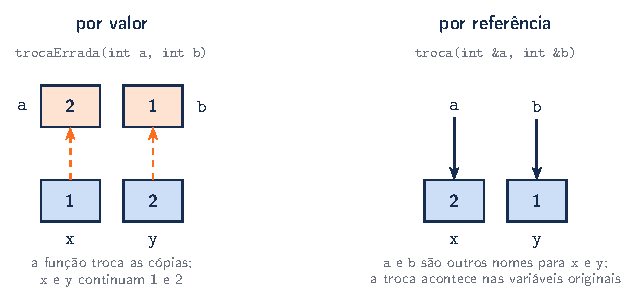
\includegraphics[width=0.9\linewidth,keepaspectratio]{imagens/capitulo-06_passagem.pdf}
\end{center}

No Portugol, a passagem por referência é indicada pela palavra \texttt{var} antes dos parâmetros:

\begin{codigo}
\begin{Verbatim}[breaklines=true, breaksymbolleft={}, fontsize=\footnotesize]
algoritmo "Troca"
var
   x, y: inteiro

procedimento troca(var a, b: inteiro)
var
   aux: inteiro
inicio
   aux <- a
   a <- b
   b <- aux
fimprocedimento

inicio
   x <- 1
   y <- 2
   troca(x, y)
   escreval(x, " ", y)        // 2 1
fimalgoritmo
\end{Verbatim}
\end{codigo}

\subsubsection{Devolvendo mais de um resultado}

O \texttt{return} devolve um único valor. Quando uma tarefa produz dois ou mais resultados, a passagem por referência resolve: a função recebe variáveis de quem chama e as preenche.

\begin{codigo}
\begin{Verbatim}[breaklines=true, breaksymbolleft={}, fontsize=\footnotesize]
#include <iostream>
using namespace std;

void dividir(int a, int b, int &quociente, int &resto) {
    quociente = a / b;
    resto = a % b;
}

int main() {
    int q, r;
    dividir(17, 5, q, r);
    cout << "17 = 5 x " << q << " + " << r << endl;
    return 0;                // 17 = 5 x 3 + 2
}
\end{Verbatim}
\end{codigo}

Como um parâmetro por referência precisa de uma variável à qual se ligar, a chamada \texttt{troca(1, 2)} não compila: não dá para trocar o conteúdo do número 1.

\subsubsection{Referência constante}

Copiar um \texttt{int} é barato, mas copiar um texto longo ou, mais adiante, um vetor com milhares de elementos, não é. Para evitar a cópia sem permitir alterações, usa-se a \textbf{referência constante}: \texttt{void saudar(const string \&nome)}. A função lê o original, sem copiá-lo, e o compilador recusa qualquer tentativa de alterá-lo.

\begin{center}
\begin{tabular}{@{}p{0.26\linewidth}p{0.3\linewidth}p{0.32\linewidth}@{}}
\toprule
\rowcolor{headergray}
\tblheader{Passagem} & \tblheader{Como se escreve} & \tblheader{Use quando} \\
\midrule
por valor & \texttt{int a} & a função só precisa do valor (o caso mais comum) \\
\rowcolor{rowgray} por referência & \texttt{int \&a} \newline Portugol: \texttt{var a} & a função precisa alterar a variável de quem chama \\
referência constante & \texttt{const string \&a} & o dado é grande e a função só vai lê-lo \\
\bottomrule
\end{tabular}
\end{center}

\subsection{6.7 Protótipos, valores padrão e sobrecarga}

\subsubsection{Protótipos}

O compilador lê o arquivo de cima para baixo, e uma função só pode ser chamada depois de ser declarada. Por isso, até aqui, as funções vieram antes do \texttt{main}. Quando se prefere o \texttt{main} no topo, para quem lê o programa ver primeiro o panorama, declara-se antes só o cabeçalho da função, terminado em ponto e vírgula. Esse cabeçalho é o \textbf{protótipo}, e a definição completa pode vir depois:

\begin{codigo}
\begin{Verbatim}[breaklines=true, breaksymbolleft={}, fontsize=\footnotesize]
#include <iostream>
using namespace std;

double areaCirculo(double raio);       // protótipo

int main() {
    cout << areaCirculo(2) << endl;    // 12.5664
    return 0;
}

double areaCirculo(double raio) {      // definição
    const double PI = 3.14159265358979;
    return PI * raio * raio;
}
\end{Verbatim}
\end{codigo}

\subsubsection{Valores padrão e sobrecarga}

O C++ tem dois recursos que o Portugol não tem. Um parâmetro pode ter um \textbf{valor padrão}, usado quando o argumento é omitido na chamada. E duas funções podem ter o \textbf{mesmo nome}, desde que os parâmetros sejam diferentes em quantidade ou tipo: é a \textbf{sobrecarga}. O compilador escolhe qual chamar pelos argumentos.

\begin{codigo}
\begin{Verbatim}[breaklines=true, breaksymbolleft={}, fontsize=\footnotesize]
#include <iostream>
using namespace std;

void linha(int tamanho = 20, char simbolo = '-') {
    for (int i = 0; i < tamanho; i++) cout << simbolo;
    cout << endl;
}

int maior(int a, int b) { return a > b ? a : b; }
double maior(double a, double b) { return a > b ? a : b; }

int main() {
    linha();             // 20 traços
    linha(5);            // -----
    linha(5, '*');       // *****
    cout << maior(3, 8) << " " << maior(2.5, 1.5) << endl;
    return 0;            // 8 2.5
}
\end{Verbatim}
\end{codigo}

Os parâmetros com valor padrão precisam ser os últimos da lista: não dá para omitir o primeiro argumento e informar o segundo.

\subsection{6.8 Um programa completo: notas da turma}

O programa abaixo refaz a análise de notas do Capítulo 5, agora dividida em subprogramas. Cada um tem uma única tarefa: \texttt{lerNota} pede uma nota até ela ser válida, \texttt{situacao} classifica uma nota e \texttt{mostrarResumo} imprime o resultado final.

\begin{codigo}
\begin{Verbatim}[breaklines=true, breaksymbolleft={}, fontsize=\footnotesize]
#include <iostream>
#include <string>
using namespace std;

double lerNota(int aluno) {
    double nota = 0;
    do {
        cout << "Nota do aluno " << aluno << " (0 a 10): ";
        cin >> nota;
    } while (nota < 0 || nota > 10);
    return nota;
}

string situacao(double nota) {
    if (nota >= 6) return "aprovado";
    if (nota >= 4) return "recuperação";
    return "reprovado";
}

void mostrarResumo(double soma, int alunos, int aprovados) {
    cout << "Média da turma: " << soma / alunos << endl;
    cout << "Aprovados: " << aprovados << " de " << alunos
         << endl;
}

int main() {
    int alunos;
    cout << "Quantos alunos? ";
    cin >> alunos;
    double soma = 0;
    int aprovados = 0;
    for (int i = 1; i <= alunos; i++) {
        double nota = lerNota(i);
        string s = situacao(nota);
        cout << "  " << s << endl;
        soma += nota;
        if (s == "aprovado") aprovados++;
    }
    if (alunos > 0) mostrarResumo(soma, alunos, aprovados);
    return 0;
}
// 3 alunos com 7, 4.5 e 3 -> aprovado, recuperação,
// reprovado; Média da turma: 4.83333; Aprovados: 1 de 3
\end{Verbatim}
\end{codigo}

Repare em uma escolha de projeto: \texttt{situacao} não mostra nada na tela, só devolve o texto. Quem decide o que fazer com ele é o \texttt{main}, que o imprime e também o usa para contar os aprovados. Separar o \textbf{cálculo} da \textbf{entrada e saída} deixa as funções mais fáceis de reaproveitar e de testar: para conferir \texttt{situacao}, basta chamá-la com 6, 5.9, 4 e 3.9, os valores nas fronteiras de cada faixa.

\subsection{Erros Comuns}

\begin{itemize}
  \item \textbf{Esquecer o \texttt{return} em algum caminho.} Uma função que não é \texttt{void} precisa devolver um valor em todos os casos. Compile com \texttt{-Wall} para ser avisado.
  \item \textbf{Chamar uma função e ignorar o resultado.} \texttt{media(n1, n2);} sozinho na linha calcula a média e a joga fora. Guarde o resultado ou use-o em uma expressão.
  \item \textbf{Esperar que a passagem por valor altere a variável.} O parâmetro é uma cópia. Para alterar o original, use \texttt{\&} em C++ ou \texttt{var} em Portugol.
  \item \textbf{Trocar a ordem dos argumentos.} A correspondência é pela posição: \texttt{dividir(5, 17, q, r)} divide 5 por 17, não 17 por 5.
  \item \textbf{Usar uma variável local fora da sua função.} Ela só existe dentro do bloco em que foi declarada.
  \item \textbf{Abusar de variáveis globais.} Qualquer função pode alterá-las, e os erros ficam difíceis de rastrear. Use parâmetros e \texttt{return}.
  \item \textbf{Chamar a função antes de declará-la.} Coloque a definição antes do \texttt{main} ou declare o protótipo no início do arquivo.
  \item \textbf{Fazer funções que fazem tudo.} Se o nome precisa de um ``e'' (\texttt{lerECalcularEMostrar}), provavelmente são três funções.
\end{itemize}
